
%% idea: mechanics model instead of optimization



%% model: cost function: congestion pricing combined with idle resource pooling
Our model is based on congestion pricing in which the cost of a
resource dynamically changes according to the load of the resource.

Another key idea is idle resource pooling that tries to put resources
into idle states as much as possible for energy saving.

The model employs convex pseudo cost functions that combines congestion
pricing with idle resource pooling.

\subsection{Pseudo Cost Functions}

\begin{figure}[thb]
\begin{center}
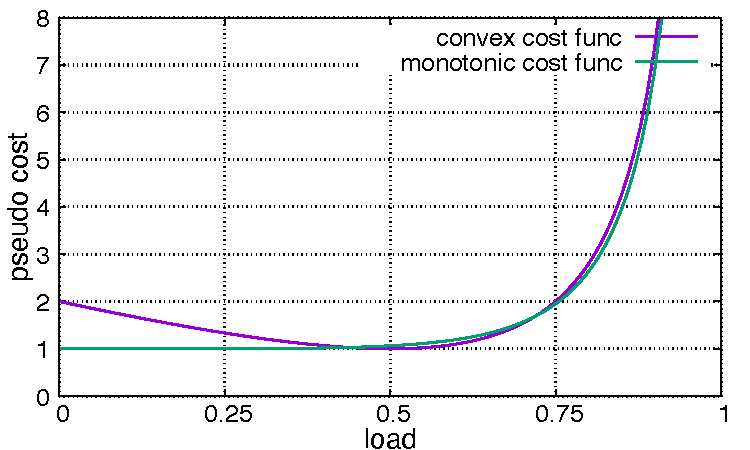
\includegraphics[width=7.5cm,clip]{costfunc.pdf}
\vspace{-2.0ex}
\caption{standard pseudo cost function}
\label{fig:std_costfunc}
\end{center}
\end{figure}

The standard pseudo cost function from the load of a resource
$\rho \in [0, 1]$ to the curresponding cost is in Figure
\ref{fig:std_costfunc}: \\

\( f(\rho) = \frac{(2\rho - 1)^{2}}{1 - \rho} + 1  \) \\

This is a convex function with the properties:
$min f(\rho) = f(.5) = 1$, and $f(0) = f(.75) = 2$.
The pseudo cost grows rapidly when $\rho \ge .75$.

The system automatically tries to keep the load of a resource in the
working range, $[0 \le \rho \le .75]$, aiming at $\rho = .5$. \\

In this model, constraints in optimization problems (e.g.,
capacity limit) are enforced by the rapid increase of the cost function when
the load approaches $1$. 

\subsubsection{Pseudo Cost Function in Action}

The behavior of the pseudo cost function is illustrated by the
following examples.

Assume a pool of equivalent resources with the standard pseudo cost
function (Figure \ref{fig:std_costfunc}).
Also, assume that micro jobs are continuousy assigned to the
system; each micro job is much smaller than the capacity of a
resource.

The initial system load $\sum \rho$ is $0$, and gradually increased
up to $2.0$, here, load $1.0$ is the capacity of a single resource.
Initially, all resources in the pool are idle, and their costs are
all $f(0)= 2$.
First, one resource $r_{0}$ is randomly selected for allocation, and it's
cost becomes lower: $f(0+) < 2$. As a result, subsequent jobs are
assigned to $r_{0}$, with lowering cost towards $\rho = .5$ and then
rising again until $\rho = .75$ where $f(.75) = 2 = f(0)$.
At this point, another resource $r_{1}$ is selected for allocation.
$r_{1}$ is preferred over $r_{0}$ as its cost becomes lower with new
allocation so that both loads move towards $\rho_{0} = \rho_{1} = .5$,
where both are balanced.
Both loads rise again until $\rho_{r_{0}} = \rho_{r_{1}} = .75$,
where the third resource $r_{2}$ kicks in.
When $\sum \rho$ reaches $2.0$, $\rho_{r_{0}} = \rho_{r_{1}} = \rho_{r_{2}} = .67$.

When the system load decreases, the process is reversed.
Assume the system load is gradually decreased from $2.0$.
After reaching $\rho_{r_{0}} = \rho_{r_{1}} = \rho_{r_{2}} = .5$,
one resource with the lowest load $\rho < .5$ becomes more expensive
than the others.
This one is less preferred for subsequent assignments, and quickly
loses the load until it becomes idle again, while the other 2 keep
$\rho = .5$. It repeats for the remaining ones.

Looking at how the number of active resources changes in a coarser
time scale,
when the number of active resources is increasing, the load of each
active resource stay at $\rho = .75$.
On the other hand, when the number of actice resources is decreasing,
the load of each active resource stay at $\rho = .5$.
In short, when all resources are equal, the system tries to maintain
the load of active resources in the range $(.5, .75)$, while keeping
idle resources as much as possible.

When resources are not equal, the behavior becomes more complex, but
the underlying mechanisms are the same.
Let's take a look at a case of two resources with the cost ratio $1:2$,
that is $f_{r_1{}}(\rho) = 2 f_{r_{0}}(\rho)$.
To activate $r_{1}$, the load of $r_{0}$ goes up to $.84$ to satisfay:
$f_{r_{1}}(0) = 4 = f_{r_{0}}(.84)$.
When $r_{1}$ is moving towards idle, the load of $r_{0}$ is $.75$ to
satisfy: $f_{r_{1}}(.5) = 2 = f_{r_{0}}(.75)$

For unequal resources in general, the required load to trigger new
resource allocation would be higher than $\rho = .75$ for the already
active ones to match the cost $f(0)$ for the new one, but the load
will not go much further as the slope of the function is steep.
Similarly, when the most expensive one among active resources becomes
idle, the load of the remaining ones stay at the matching cost at
$f(.5)$ for the deactivating one. 

The system could be stabilized at local minimum (e.g., cannot activate
a resource with the minimum cost).
However, our goal is not to achieve the theoretical optimum but to
enable loose automatic distributed load balancing.

\subsubsection{Variations}

The operator can control the resource utilization by modifying the cost
function of the resource.

\begin{description}
\item[lowering/raising utilization] by raising/lowering the pseudo cost. \\
  $f'(\rho) = f(\rho) + \Delta$ \\
or \\
  $f'(\rho) = (1 \pm \Delta)f(\rho)$ \\
The difference from the original is milder for the former additive
form; the difference of the latter multiplicative form rapidly grows
as the load moves away from the center.

\item[increaing idle-state] by raising the the cost for light load.
\item[premium service] can be realized by lowering the target load so
  that the job runs on lightly loaded resources. \\
  $f'(\rho) = f(\rho - \Delta)$
\item[equal load-balancing] without idle resource pooling can be
  achieved by simple monotonic functions, e.g.,
  $f(\rho) = \frac{\rho^{2}}{1 - \rho} + 1$.
\item[hierarchical model] will be discussed later in Section XX.
\end{description}

\subsection{Jobs}

micro job $J(p, q, r, s)$	\\
$p$: $\sharp$ of micro containers	\\
$q$: frontend communications (Mbps)	\\
$r$: backend communications (Mbps)	\\
$s$: $\sharp$ of time slots (sec)	\\

For simplicity, we do not distinguish directions of communications for $q$ and $r$.

Optionally, a job can specify weights for the cost calculation with $p$, $q$, $r$:
e.g., an interactive job may raise the weight for the frontend
communication to place the job close to the user.

\subsection{Job Assignment}

To instantiate a micro job requested from a user, the system allocates
the required resource for $J$: $p$, $q$ and $r$ for duration $s$.

%%pseudo cost: is used to solve the resource allocation problems;
%%it is not a real cost such as service charges. \\
%%$f(r, t, s)$: cost function for resource $r$ (micro container $P$ or link $L$ )
%%at time $t$ for $s$ time slots. \\
%%$f(r, t, s)$ is a function of the load of $r$, $\rho_{r}$ at $t$. \\
%%$f(r)$: we omit $t$ and $s$ for $t=t_{current}$ and for a unit time (1 sec)  \\


resource unit: one micro container for $P$, 1Mbps for $L$. \\
$H(j, i)$: CPU cost to run $j$ at $i$ \\
\( H(j, i) = f(i) \cdot p \)	\\
$G(j, i, m, o)$: communication cost to run $j$ at $i$ between $m$ and $o$. \\
$path(m,i)$: a set of links in the best path from $m$ to $i$. \\
\( G(j, i, m, o) = \sum_{l \in path(m,i)} f(l) \cdot q + \sum_{l \in path(i,o)} f(l) \cdot r \) \\
pseudo cost $E$ to host job $j$ for a unit time at node $i$ for user $m$, data obj $o$: \\
\( E(j, i)  =  H(j,i) + G(j,i,m,o) =  f(i) \cdot p + \sum_{l \in path(m,i)} f(l) \cdot q + \sum_{l \in path(i,o)} f(l) \cdot r \) \\
(For now, we assume only one user and one data object per job) \\
To assign Job $j$, we simply find: \\
\(  argmin_{i} \: E(j, i)   \)  \\
and then, assign $j$ to $i$. \\

  
\subsection{Misc}

The load of a resource can be measured in a number of ways.  Most
resources have some form of load report functions built-in.
A load value does not need to be precise, and a rough approximation is
enough for resource management.



